\chapter{Wprowadzenie}

Widzenie maszynowe jest jedną z~najprężniej rozwijających się
dziedzin z~pogranicza algorytmiki, optymalizacji, przetwarzania obrazów,
przetwarzania sygnałów, statystyki oraz szeroko pojętej sztucznej
inteligencji jeżeli chodzi o~zagadnienia informatyczne w~ostatnich
latach. Trudno zdefiniować pojęcie widzenia maszynowego w~jednym
zdaniu. Niektórzy twierdzą, że jej zadaniem jest podejmowanie
decyzji, klasyfikowanie oraz opisywanie fizycznych obiektów
i~scen na podstawie obrazów \cite{ShapiroStockman200102}.
Można też natknąć się na stwierdzenie, że wizja komputerowa 
grupuje zagadnienia związane z~ekstrakcją danych numerycznych -
numerów, współrzędnych, symboli i~ciągów znaków - zawartych w~obrazach
\cite{morris2004computer}. Jest to dziedzina niezwykle pojemna. 
Interdyscyplinarność czyni próbę wymienienia zagadnień z~nią związanych,
bez pominięcia jakiejś istotnej gałęzi, niemal niemożliwą. 
W~celu zobrazowania złożoności i~rozległości zakresu jaki wiąże się
z~tym zagadnieniem posłużono się ilustracją \cite{wiki:computervision}, 
którą zamieszczono poniżej - rysunek 
\ref{fig:int_cv_inter_discip}.

\begin{figure}[!h]
    \centering
    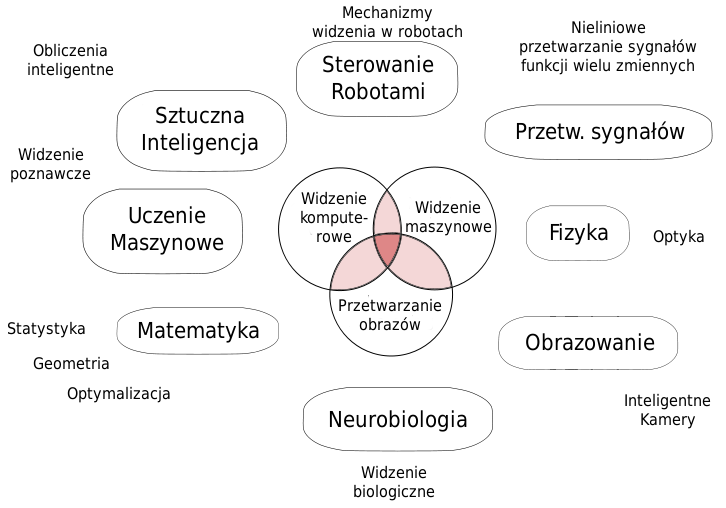
\includegraphics[width=0.9\textwidth]{img/int_cv_inter_discip}
    \caption{Powiązanie wizji komputerowej z~innymi dziedzinami}
    \label{fig:int_cv_inter_discip}
\end{figure}

Celem tej pracy jest przygotowanie działającej implementacji
algorytmu odczytującego numer zawarty we froncie nadjeżdżającego
autobusu na urządzeniu mobilnym z~systemem android. Przygotowaniem
do tego przedsięwzięcia był przegląd dostępnych metod wykrywania
obiektów w~obrazach. Przeanalizowano również dostępne biblioteki 
i~narzędzia pod kątem odczytu tekstu ze sceny naturalnej.

Scenariusz wykorzystania aplikacji zaprezentowano na rysunku
\ref{fig:int_use_case_diag}.

\begin{figure}[!h]
    \centering
    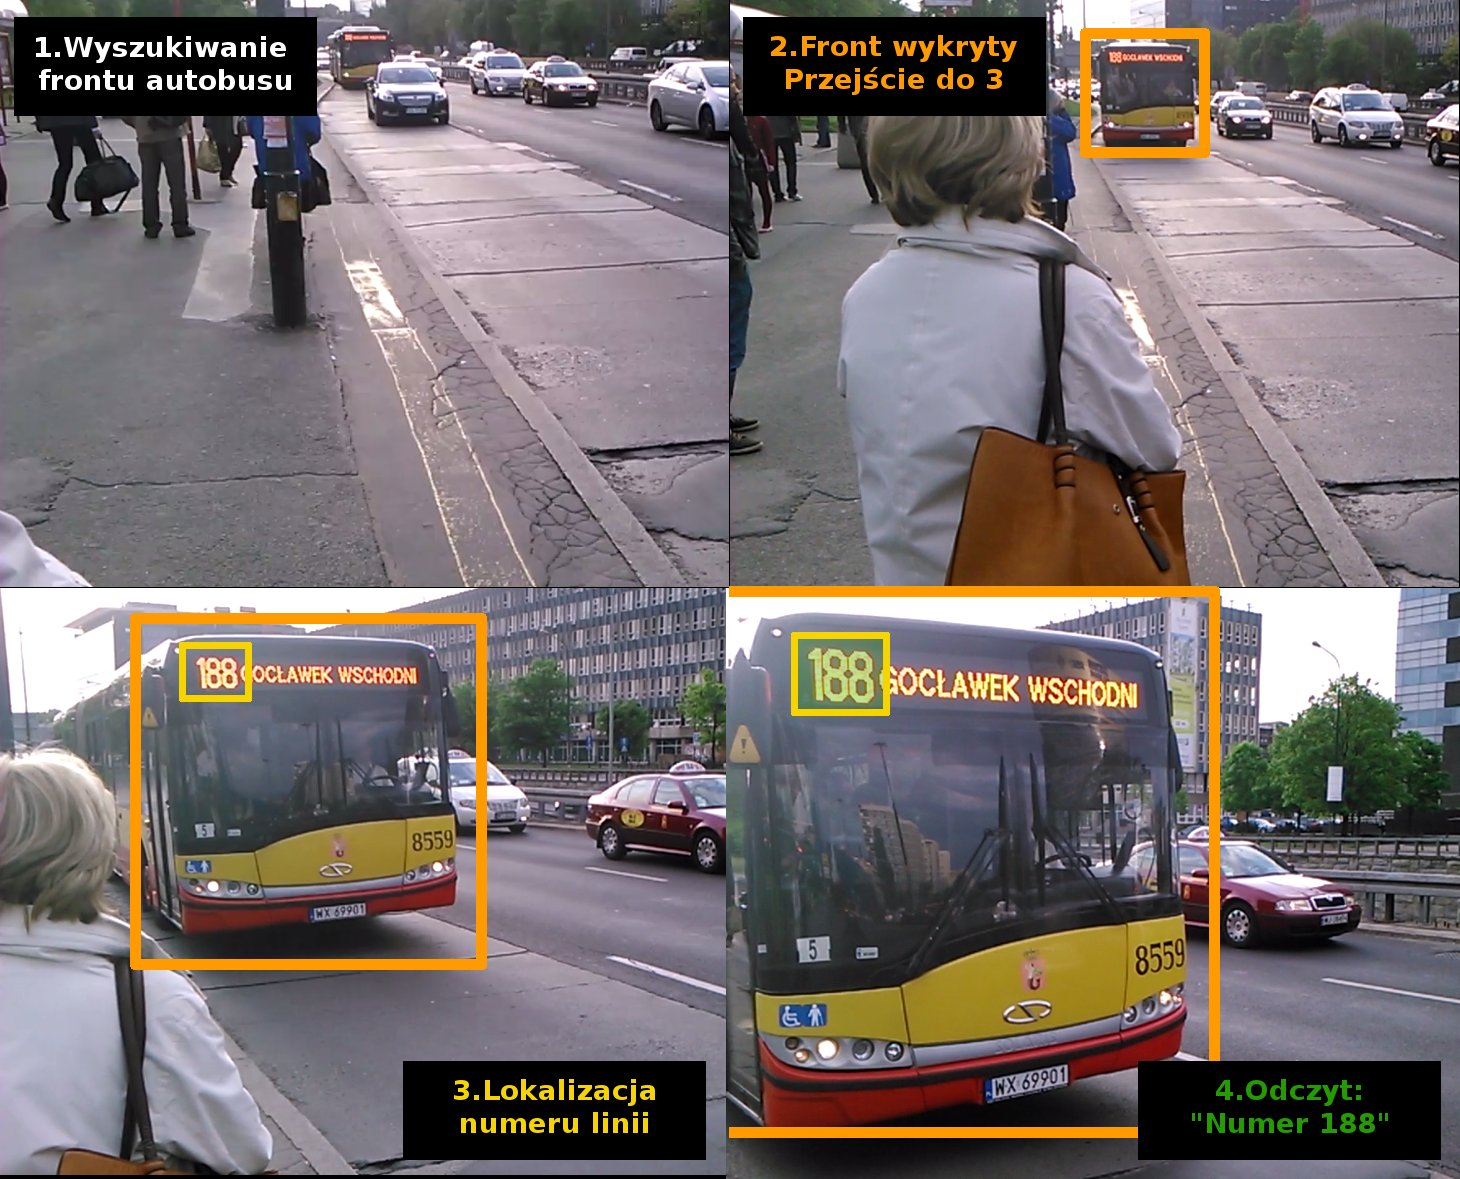
\includegraphics[width=0.9\textwidth]{img/int_use_case_sequence}
    \caption{Diagram przedstawiający przypadek użycia proponowanej aplikacji}
    \label{fig:int_use_case_diag}
\end{figure}

Użytkownik - osoba niewidoma - stojący na przystanku autobusowym powinien
być zwrócony twarzą do nadjeżdżających samochodów. Trzymając
telefon tak aby kamera zbierała klatki obrazu
z~najbliższych chodnikowi pasów ruchu (co najmniej z~zatoki autobusowej)
użytkownik uruchamia aplikację. Następuje wejście aplikacji w~tryb
wyszukiwania frontu. W~momencie odnalezienia frontu aplikacja
przełącza się w~tryb odczytywania numeru sygnalizując o~tym użytkownika.
Próba odczytania może się powieść lub nie dlatego aplikacja może
zakończyć ten etap na wiele różnych sposobów:

\begin{itemize}
	\item numer został jednoznacznie odczytany - komunikat z~odczytanym 
		numerem linii,
	\item numer odczytany, lecz jest kilku prawdopodobnych kandydatów - 
		komunikat mówiący o~niepewności odczytu zwracanych jest
		kilka pierwszych najbardziej prawdopodobnych numerów,
	\item odczyt błędny lub brak wyraźnych faworytów - komunikat
		o~niemożliwości odczytania numeru,
	\item niedostateczna liczba pobranych danych - komunikat 
		o~prawdopodobnej utracie obiektu - wyjście frontu
		poza kadr, zasłonięcie przez przeszkodę itp.
\end{itemize}

Po udanym lub nieudanym odczycie aplikacja przechodzi w~stan spoczynku,
a~użytkownik ma możliwość - poprzez kliknięcie
elementu w~odpowiednim menu - uruchomić
ponownie tryb wyszukiwania frontu.

\section{Zakres pracy}

W~pracy zawarto przegląd dostępnych implementacji związanych
z~detekcją i~identyfikacją obiektów. W~drugim rozdziale 
wprowadzono obowiązujące
w~tym opracowaniu definicje detekcji i~identyfikacji. 
W~pierwszym podrozdziale omówiono metody wykrywania obiektów.
Skupiono się
głównie na istniejących rozwiązaniach, algorytmach, narzędziach 
i~bibliotekach. Duży nacisk położono na bibliotekę OpenCV. 
Jest ona bowiem dostępna na komputery PC, systemy Windows oraz Linux, 
urządzenia
mobilne, a~także system Android. Ze względu na bogactwo zaimplementowanych
funkcji, algorytmów i~narzędzi pomocniczych jest pozycją numer 
jeden w~zestawie każdego eksperymentatora. Zaskakująco dobre
rezultaty skłoniły do opisania biblioteki OpenTLD. Jednak brak
implementacji na system Android sprawił, że była ona traktowana raczej jako
ciekawostka. Drugi podrozdział to krótka wzmianka o~metodach
rozróżniania obiektów.

W~trzecim rozdziale przedstawiono nieudaną próbę implementacji
środowisk: deweloperskiego i~testowego. Niepowodzenie
spowodowane było niekonsekwencją
i~zbytnim skupieniem się na szczegółach w~momencie gdy ani
architektura rozwiązania końcowego, ani kluczowe elementy wymagające
automatyzacji nie były jeszcze znane.

Kolejny - czwarty rozdział - opisywał wykonane doświadczenia
i~eksperymenty. W~pierwszej kolejności zamieszczono opis 
eksperymentów, których wyniki były niezadowalające. Metody testowane 
w~tym rozdziale nie zostały wykorzystane w~rozwiązaniu końcowym.
Podczas prób z~odczytywaniem
tekstu oprócz biblioteki OpenCV wzięto pod uwagę silnik 
OCR o~nazwie Tesseract. W~obu przypadkach
czynnikami wiodącymi podczas dokonywania wyboru była zarówno jakość
jaki i~cena oferowanych rozwiązań. Oba narzędzia
były darmowe, a~licencja umożliwiała implementację komercyjną 
bez uiszczania
jakichkolwiek opłat. Dodatkowym atutem w~przypadku narzędzi Tesseract
było wsparcie rozwoju narzędzia przez firmę Google, oraz tak samo jak 
w~przypadku OpenCV, istniejący port na system Android.
W~podsumowaniu rozdziału czwartego zamieszczono opis prób kompletnej
implementacji. Uruchamianej jednak jeszcze na komputerze stacjonarnym.

Piąty mini-rozdział powstał w~wyniku implementacji rozwiązania na 
systemie docelowym. Opisano pierwsze próby aplikacji deweloperskiej
uruchomionej na dwóch podobnej klasy urządzeniach. Na końcu
zaprezentowano wyniki doświadczeń z~aplikacją demonstracyjną,
która zawierała już niemal całą zakładaną funkcjonalność.

W~opracowaniu brakuje wyników rzetelnie przeprowadzonych testów
skuteczności (ilości i~dokładności) oraz wydajności zaimplementowanej 
aplikacji, a~także poszczególnych jej elementów. Próby 
przygotowania automatów do mierzenia skuteczności i~wydajności
były podejmowane równolegle do poszukiwań odpowiednich metod
wykrywania i~odczytywania numeru. Brak wiedzy o~końcowym wyglądzie
rozwiązania spowodował, że były one zupełnie nieadekwatne i~nieprzystosowane
do postawionego zadania. Testy dla próbek w~liczbie kilku tysięcy sztuk
trwały długo (kilka godzin), a~wyniki nie dość, że nie dawały prawdziwego
obrazu sytuacji potrafiły wręcz wprowadzić w~błąd.
Nie obyło się bez naocznej interpretacji wybranych przypadków testowych. 
Ostatecznie więc wykonano testy manualnie. Co było główną przyczyną
bardzo małej liczby wykorzystanych próbek oraz niskiej
wartości otrzymanych wyników w~ogóle.
